\chapter{Experiment}
\label{ERef}
Er hebben doorheen het jaar, verschillende experimenten plaats gevonden. We zijn begonnen met meer eenvoudige experimenten en zijn ge\"eindigd met de moeilijkere experimenten. We bespreken de experimenten in chronologische volgorde. Na de beschrijving en de uitwerking van de verschillende experimenten worden conclusies getrokken uit de resultaten en de berekeningen. Met de conclusies van de vorige experimenten werd dan ook rekening gehouden bij de uitvoering van de volgende experimenten. Er zijn zes verschillende experimenten gebeurd. We beginnen met opslaan van beelden in sectie\ref{ERefOvB}. Vervolgens detecteren we het uit het bed stappen \ref{ERefDUB}. Dit deel is opgesplitst in twee verschillende experimenten, namelijk een eerst poging \ref{ERefDUBEP} en een tweede poging \ref{ERefDUBTP}. Tijdens het volgende experiment hebben we met live beelden \ref{ERefELB} gewerkt. Daarna hebben we geprobeerd het restwarmte probleem te verkleinen \ref{ERefRWV},als voorlaatste experiment hebben we de pixelwaarde zonder normalisatie bestudeerd \ref{ERefPZN}. Bij het laatste experiment zijn we kijken of we aan de hand van de locatie van het hoofd iets kunnen zeggen over het uit bed stappen \ref{ERefHGD}.

\section{Opslaan en ophalen van beelden}
\label{ERefOvB}
Dit eerste experiment bespreken we in 4 verschillende delen. We beginnen met te verklaren wat ons doel was van het experiment \ref{ERefOBD}, daarna bespreken we de gebruikte klassen, methodes en de flowchart \ref{ERefOBF}. Vervolgens verklaren we de specifieke uitwerking van het experiment \ref{ERefOBU}. Als laatste trekken we onze conclusies \ref{ERefOBB}.

\subsection{Doel van het experiment}
\label{ERefOBD}
Het doel van dit experiment is het opslagen van beelden en het ophalen van beelden. Dit om dan achteraf verschillende processen over de beelden te laten lopen en zo te zien welke de beste resultaten geeft. 

\subsection{Gebruikte klassen en flowchart}
\label{ERefOBF}
\begin{figure}[hbp]
	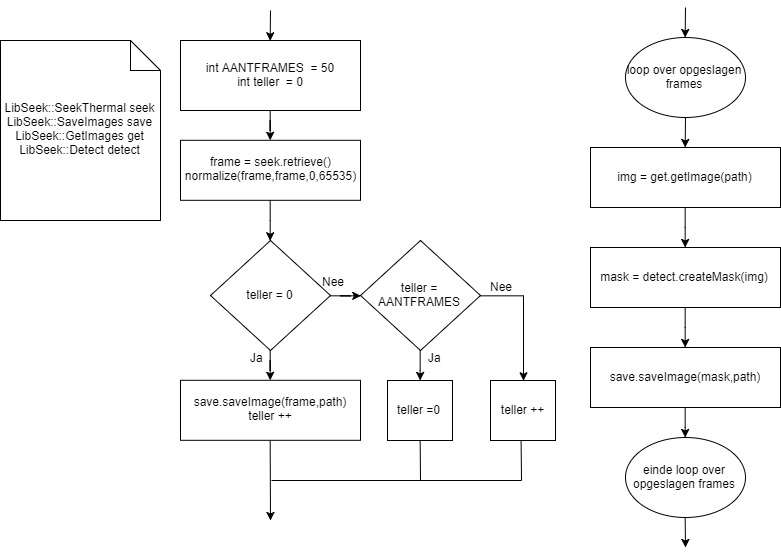
\includegraphics[scale=0.45]{FlowChart_EersteExperiment}
	\caption{Flowchart eerste experiment, naamgeving objecten (links), opslaan afbeelding (rechts) en ophalen afbeelding en masker cre\"eren (rechts)}
	\label{imgFCEEx}
\end{figure}
Voor dit experiment werd voornamelijk de gekregen code gebruikt om de code met de computer in te lezen. Vervolgens maken we gebruik van de klassen SaveImages \ref{mRefSIm}, GetImages \ref{mRefGIm} en Detect \ref{mRefDet}. De opeenvolging van de gebruikte methodes vindt u terug in de flowchart, deze ziet u in figuur \ref{imgFCEEx}.Zoals u ziet bestaat het flowchart uit drie delen. Links ziet u de naamgeving voor de verschillende objecten. Dit zodat u beter begrijpt welke methodes we juist bedoelen in de flowchart. In het midden ziet u het flowchart voor het opslaan van de frames. We gaan de waarde van teller vergelijken om de frames maar om de 50 keer op te slagen. Als teller niet 0 of 50 is, wordt er 1 bij geteld, bij 0 wordt het frame opgeslagen en wordt de teller met 1 vergroot, is teller 50, dan gaan we de waarde van teller terug 0 maken, zo wordt het volgende frame weer opgeslagen. Links ziet u de flowchart voor het ophalen van de afbeelden en het cre\"eren van het masker. We gaan elke afbeelding van het frame \'{ee}n voor \'{ee}n ophalen met getImage, vervolgens cre\"ren we let createMask het masker voor de opgehaalde afbeelding. Als laatste gaan we dan het masker wegschrijven.


\subsection{Uitvoering experiment en resultaten}
\label{ERefOBU}
\begin{figure}[hbp]
	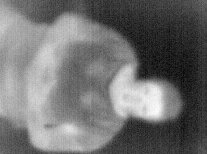
\includegraphics[scale=0.65]{EersteExperiment_img0}
	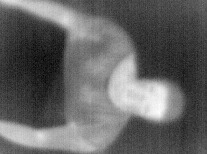
\includegraphics[scale=0.65]{EersteExperiment_img2}
	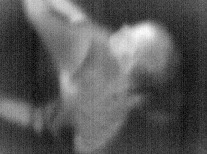
\includegraphics[scale=0.65]{EersteExperiment_img3}
	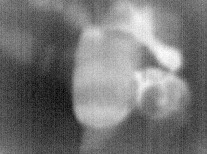
\includegraphics[scale=0.65]{EersteExperiment_img6}
	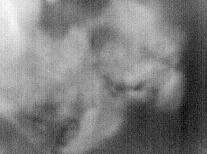
\includegraphics[scale=0.65]{EersteExperiment_img9}
	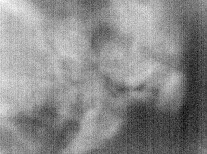
\includegraphics[scale=0.65]{EersteExperiment_img10}
	\caption{Opgeslagen beelden in eerste experiment}
	\label{imgEEx}
\end{figure}
Tijdens het eerste experiment hebben we overdag met behulp van de camera \ref{mRefSTh} beelden genomen van een persoon in bed. We slaan het frame maar om de 50 opgehaalde frames op. Dit omdat anders de verschillen tussen de opgeslagen frames niet groot genoeg was. We wensten beelden van verschillende lighoudingen.  Deze beelden kunnen we dan gebruiken voor het maken van bijvoorbeeld het masker en het verder afwerken van de detectie. Zo kunnen we nagaan of er een goede segmentatie gebeurde vooraleer we begonnen met het maken van beelden gedurende een volledige nacht.\\
De beelden die zijn opgeslagen tijdens dit eerste experiment vindt u terug in figuur \ref{imgEEx}. Zoals u ziet hebben we zoveel mogelijk verschillende slaaphoudingen aangenomen. We zien eveneens een verschil in de afbeeldingen bij gebruik van een deken. De twee laatste afbeeldingen zijn van het leeg bed net nadat de foto's getrokken zijn. \\
Tijdens dit experiment hing de camera boven het bed. Een schets van het zijaanzicht van de situatie vindt u in afbeelding \ref{imgEEx2}. De oranje rechthoeken zijn de muren, plafond en grond van de kamer. Het paarse driehoekje is de camera. De camera hing boven het hoofdeinde van het bed, ongeveer in het midden van de breedte van het bed. \\
De resultaten spraken ook voor zich, de foto's werden opgeslagen in de gewenste map. Verder zien we dat de persoon duidelijk te scheiden is van de achtergrond. Door gebruik te maken van deze afbeeldingen, zochten we ook naar de ideale waarde voor de drempelwaarde om het masker te cre\"eren, zoals reeds besproken is bij de verschillende methodes van de klasse Detect \ref{mRefDet}. Een voorbeeld van een gecre\"eerd masker kan u zien in figuur \ref{imgCMa}.
\begin{figure}[hbp]
	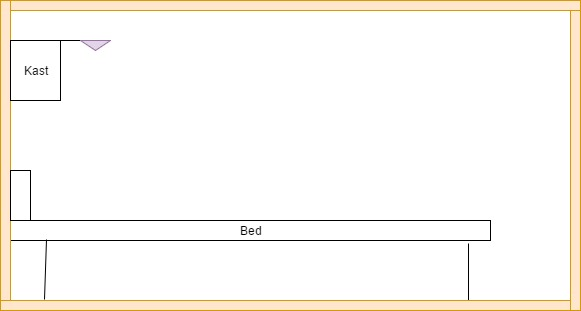
\includegraphics[scale=0.5]{SchetsExperiment1}
	\caption{Schets van de situatie in het eerste experiment}
	\label{imgEEx2}
\end{figure}

\subsection{Besluiten uit het experiment}
\label{ERefOBB}
\begin{figure}[hbp]
	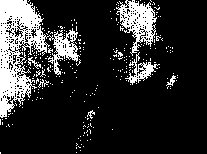
\includegraphics[scale = 0.75]{EersteExperiment_mask10}
	\caption{Verkregen masker voor leeg opgewarmd bed}
	\label{imgCOB}
\end{figure}
Bij het bekijken van de opgeslagen beelden \ref{imgEEx} vielen er ons drie zaken op op. Ten eerste, als er een deken over de persoon ligt, was hiervan enkel nog het hoofd en eventueel ook armen zichtbaar. Ten tweede warmt het bed zeer snel op. Zo kan je in de laatste frames een leeg bed zien nadat de persoon er voor ongeveer 10 minuten had ingelegen. Dit is ook al zeer licht en kan leiden tot valse persoon detecties, dit is natuurlijk niet wenselijk voor ons experiment. Een voorbeeld van een verkregen masker voor een leeg opgewarmd bed, ziet u in figuur \ref{imgCOB}.  Hiervoor gaan we dus in de komende experimenten een oplossing moeten zoeken. Ten derde zien we ook dat we de camera verder van het bed moeten plaatsen om het volledige bed en persoon in het beeld te krijgen. Ook ziet u, dat als de persoon eerst op de zij heeft gelegen en gedraaid is, een lichter vlak op de plaats waar de persoon voordien lag. Een tweede mogelijk probleem dat optreedt is dat als je het masker cre\"eert, je de lichaamsdelen die bedekt worden door een deken maar ook door bijvoorbeeld een kledingstuk zoals pyjama soms mist. Hierdoor zou het kunnen dat mogelijke aanstalten om uit het bed te stappen niet gedetecteerd worden. \\ 
Verder maakt de camera ook een klikgeluidje elke keer als er een frame gemaakt wordt. Dit kunnen sommige mensen hinderlijk vinden als ze hier mee moeten slapen. Dit kan enkel opgelost worden door een andere camera te gebruiken. Het klikgeluidje wordt gemaakt elke keer dat er een frame wordt opgeslagen. We kunnen natuurlijk ook zien of we het aantal frames dat genomen wordt kunnen verkleinen. Hierdoor gaat ook het aantal klikjes verkleinen. Als we bijvoorbeeld 1 frame per seconde nemen, wordt dit qua geluid gelijk aan het tikken van een klok.

\section{Detecteer uit bed stappen}
\label{ERefDUB}
Net zoals bij het voorgaande experiment \ref{ERefOvB} bespreken we ook dit tweede experiment in vier verschillende delen. We beginnen met het doel van het experiment \ref{ERefDBD} en het verduidelijken van de gebruikte klassen en methodes \ref{ERefDBK}. Vervolgens verklaren we de uitwerking \ref{ERefDBV} en de verkregen resultaten. Als laatste nemen we een paar besluiten uit de verkregen beelden \ref{ERefDBB}.

\subsection{Doel van het experiment}
\label{ERefDBD}
Het doel van het experiment is te bepalen of het mogelijk is te detecteren wanneer een persoon uit bed stapt en het ontwikkelen van de algoritmes die hiervoor nodig zijn.

\subsection{Gebruikte klassen en flowchart}
\label{ERefDBK}
Er wordt hier verder gebouwd op het voorgaande experiment \ref{ERefOvB}. Daarom maken we gebruik van dezelfde drie klassen, namelijk: SaveImages \ref{mRefSIm}, GetImages \ref{mRefGIm} en Detect \ref{mRefDet}. Hiernaast wordt tijdens dit experiment ook gebruik gemaakt van de klasse Bed \ref{mRefBed}. Het flowcharts van de experimenten zoals weergegeven in figuur \ref{imgFCDUBEP} en figuur \ref{imgFCDUBTP} tonen de opeenvolging van de gebruikte methodes.

\subsection{Verklaring uitwerking van het experiment}
\label{ERefDBV}
\begin{figure}[hbp]
	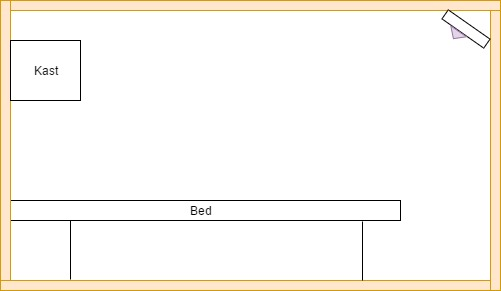
\includegraphics[scale=0.6]{SchetsExperimentTwee}
	\caption{Schets van het tweede experiment}
	\label{imgTEx}
\end{figure}
Eens de persoon uit de beelden gehaald kon worden. Hebben we nieuwe beelden gemaakt. Dit waarbij de hoeken van het bed gedefinieerd werden door middel van de constructor met een afbeelding \ref{mRefBed}. Daarna maakte de persoon verschillende keren aanstalten om uit het bed te stappen en hebben we nagegaan dat ons programma de juiste kant kan detecteren. \\
Voor dit experiment werd een nieuwe opstelling gemaakt. Een schets hiervan vindt u in figuur \ref{imgTEx}. In deze figuur \ref{imgTEx} zijn de oranje rechthoeken de muren, plafond en vloer. De camera is eveneens het paarse driehoekje. We voegen eveneens een paar voorbeelden toe van gemaakte beelden tijdens dit experiment, deze kan u zien in figuur \ref{imgTEx1}. \\
Dit experiment is op twee verschillende manieren uitgevoerd. Dit omdat we niet tevreden waren met de resultaten die we de eerste keer verkregen. We bespreken eerst de eerste poging en vervolgens de tweede poging. 
\begin{figure}[hbp]
	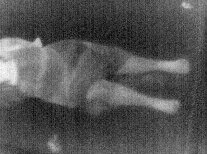
\includegraphics[scale=0.85]{TweedeExperiment_img0}
	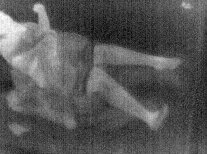
\includegraphics[scale=0.85]{TweedeExperiment_img4}
	\caption{Voorbeelden van opgeslagen afbeeldingen tijdens tweede experiment}
	\label{imgTEx1}
\end{figure}

\subsubsection{Eerste poging}
\label{ERefDUBEP}
\begin{figure}[hbp]
	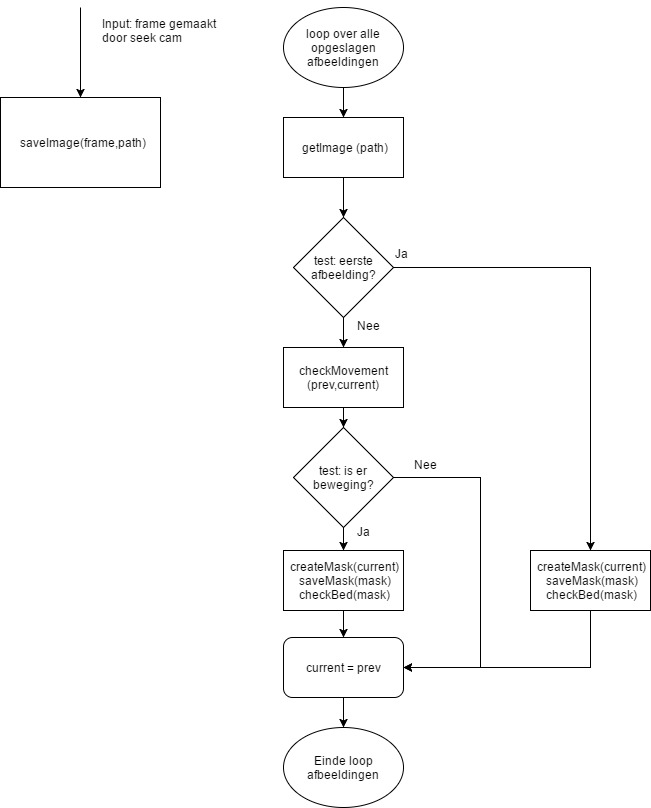
\includegraphics[scale=0.45]{FlowChart_DetectUitBed_EerstePoging}
	\caption{Flowchart eerste poging detectie uit bed stappen}
	\label{imgFCDUBEP}
\end{figure}
Om het idee achter dit experiment te verduidelijken, voegen we een flowchart toe met daarin de gebruikt methodes om tot onze resultaten te komen, dit flowchart vindt u terug in figuur \ref{imgFCDUBEP}. We houden hier wel rekening met beweging om rekentijd de besparen. Maar we controleren nergens of de oppervlakken in het masker die het alarm gaan triggeren wel bewegende delen zijn of onderdelen van de achtergrond. De gebruikte methodes worden allemaal besproken in de sectie code \ref{mrefCod}

\subsubsection{Tweede poging}
\label{ERefDUBTP}
\begin{figure}[hbp]
	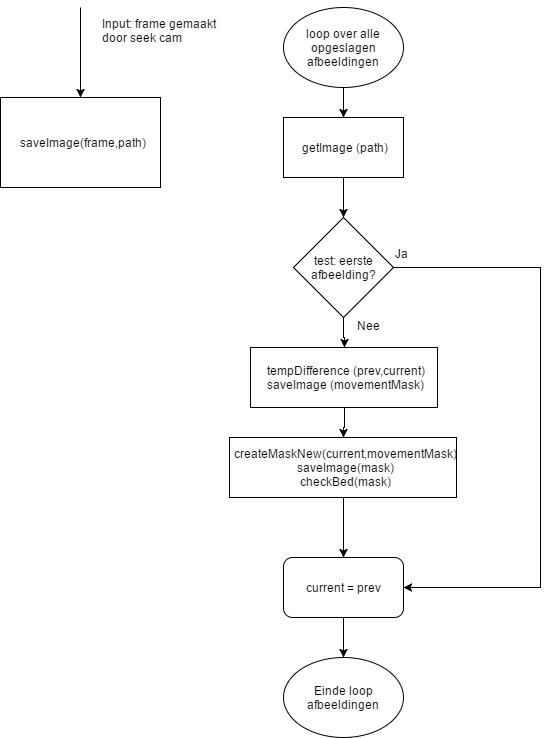
\includegraphics[scale=0.45]{FlowChart_DetectUitBed_TweedePoging}
	\caption{Flowchart tweede poging detectie uit bed stappen}
	\label{imgFCDUBTP}
\end{figure}
Nadat we onze conclusies hebben getrokken uit de eerste poging van ons experiment \ref{ERefDUBEP}, hebben we onze code aangepast. Het flowchart van deze aanpassingen vindt u in figuur \ref{imgFCDUBTP}. Het grootste verschil is dat we hier een temporeel verschil berekenen. Dit wordt opgeslagen als bewegingsmasker. Hierdoor gaan warme punten in de achtergrond, het alarm niet meer triggeren. De gebruikte methodes worden besproken in \ref{mrefCod}.

\subsection{Besluiten na de experimenten en resulaten}
\label{ERefDBB}
In dit deel bespreken we de conclusies die we hebben getrokken uit het detecteren van het uit bed stappen. De conclusie over dit stukje wordt in twee delen gesplitst. Dit omdat de resultaten van de gebruikte code in het eerste deel niet volstaat, daarna hebben we een paar aanpassingen in onze code gemaakt, de conclusies die we trekken na het toepassen van deze nieuwe code wordt als laatste besproken.

\subsubsection{Eerste poging}
\begin{figure}[hbp]
	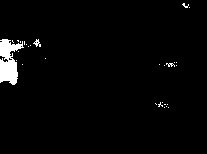
\includegraphics[scale = 0.75]{MaskTweedeExperiment_img0}
	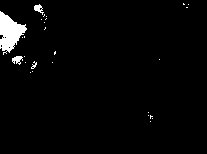
\includegraphics[scale = 0.75]{MaskTweedeExperiment_img4}
	\caption{Verkregen masker voor twee voorbeelden bij experiment twee}
	\label{imgCDUB}
\end{figure}
Bij het bekijken van de resultaten van het tweede experiment, valt bij het maken van de maskers op dat er een lichtere vlek (recht bovenaan), ook mee gedetecteerd wordt, dit is echter geen deel van een persoon. De maskers ziet u in figuur \ref{imgCDUB}.
Hierdoor krijgen we steeds de melding dat de persoon uit het bed probeert te stappen langs de rechterzijde. Dit is natuurlijk een fout. Een mogelijke oplossing voor dit probleem is eerst detecteren welke pixels verandert zijn, daar is dus een beweging. Vervolgens kunnen we voor de bewogen pixels kijken welke warm genoeg zijn om tot de persoon te behoren. Zo kunnen we deze valse detecties vermijden. Hierdoor gaat de computer wel veel meer moeten rekenen.

\subsubsection{Tweede poging}
Nadat we eerst het temporeel verschil berekenen voor we het masker maken van de lichaamswarmte op de infraroodbeelden, kunnen we door gebruik te maken van de setSidesOfBed methode van de klasse Bed bepalen langs welke kant de persoon uit het bed probeert te stappen. Als de persoon binnen de randen van het bed blijft wordt er None terug gegeven. Indien de randen van het bed wel wordt overschreven, wordt links of rechts (naargelang langs welke kant de rand wordt overschreven) afgedrukt op het scherm. Uit deze tweede poging van dit experiment kunnen we besluiten dat de detectie van langs welke zijde de persoon uit het bed stapt correct werkt. Het meten van de tijd dat een persoon weg blijft, is momenteel nog onmogelijk door de restwarmte die we nog zien in onze beelden. Een mogelijke oplossing hiervoor wordt in een volgend experiment aangeboden. 

\section{Experiment met live beelden}
\label{ERefELB}
De totale bespreking van het experiment op live beelden wordt uit gelegd in drie verschillende delen. We beginnen met te verklaren wat het doel \ref{ERefLBD} van dit experiment was, hierna bespreken we de opbouw en de uitwerking van het experiment \ref{ERefLBV}. Als laatste bespreken we de besluiten die we trekken uit dit experiment.

\subsection{Doel van het experiment}
\label{ERefLBD}
Het doel van dit experiment is na te gaan of we de veranderingen in de beelden snel genoeg detecteren. We gaan dus testen of de detectie van langs welke zijde er aanstalten gemaakt wordt om uit bed te stappen ook ogenblikkelijk gebeuren. 

\subsection{Uitwerking van het experiment}
\label{ERefLBV}
We  hebben ons systeem aangesloten op de camera en live beelden verwerkt. De proefopstelling is het zelfde gebleven als bij het vorige experiment \ref{ERefDUB}. Een schets hiervan ziet u in figuur \ref{imgTEx}. Tijdens dit experiment is er een persoon in het bed gaan liggen en heeft een paar keer gedaan als hij uit het bed wou stappen. Terwijl op het scherm in het oog werd gehouden of de computer de juiste detecties werden gemaakt.

\subsection{Besluiten na het experiment}
Uit dit experiment kunnen we besluiten dat het systeem werkt. Vanaf er een arm of een been uit het bed wordt gestoken wordt er een melding gegenereerd met de juiste zijde. Het genereren van deze melding gebeurt vrijwel onmiddellijk. Kleding en deken vormen hier nog het grootste probleem. Als het lichaam bedekt is, wordt het door het masker niet gedetecteerd. Hierdoor zouden er evenementen gemist kunnen worden. Verder loopt het ook mis als er een persoon in het bed heeft gelegen en er uit stapt. De camera detecteert dan de restwarmte van het bed en gaat doen alsof er wel nog een persoon in ligt. Zoals reeds eerder is aangehaald, wordt hiervoor in een volgende experiment een oplossing gezocht.
 
 \section{Verkleinen van het restwarmte probleem}
 \label{ERefRWV}
 Het doel van het experiment wordt als eerste besproken \ref{ERefRVD}, dit wordt gevolgd door een verduidelijking van de uitwerking van het experiment \ref{ERefRVV}. Als laatste worden de resultaten en de besluiten besproken \ref{ERefRVB}.
 
 \subsection {Doel van het experiment}
 \label{ERefRVD}
 Zoals de naam van het experiment al laat vermoeden, was het doel van dit experiment om het probleem van de restwarmte op te lossen. Dit zodat ons systeem beter zou werken en het ook mogelijk wordt om te bepalen hoelang een persoon uit het bed is. 
 
 \subsection{Uitwerking van het experiment}
 \label{ERefRVV}
 De uitwerking lijkt veel op die van de tweede poging van detectie uit bed stappen \ref{ERefDUBTP}. Het grootste verschil is dat we hier de aangepaste versie van het temporeel verschil, methode tempDifferenceNew van de klasse detect \ref{mRefDet}, gebruiken in plaats van het temporeel verschil, methode tempDifference van de zelfde klasse. Indien u wenst, kan u voor de verduidelijking ook terug kijken naar de flowchart van de tweede poging van detectie uit bed stappen ,figuur \ref{imgFCDUBTP}. Het verschil tussen de twee methodes van het temporeel verschil is dat we in de nieuwe versie niet gaan zien waar de pixelwaarde niet gelijk gebleven is, maar ook waar de pixelwaarde gestegen is. Dit omdat we willen weten waar nu wel een persoon is en voordien niet. Omdat te kamertemperatuur lager is dan de lichaamstemperatuur van een persoon, volstaat het om te kijken naar de pixels waar de temperatuur is gestegen. 
 
 
 \subsection{Bespereking van de resultaten en besluit na het experiment}
\label{ERefRVB}
\begin{figure}[hbp]
	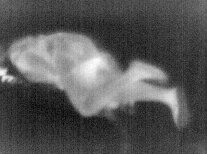
\includegraphics[scale = 0.75]{VierdeExperiment_frameJuist}
	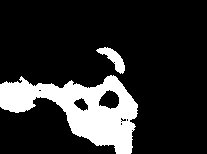
\includegraphics[scale = 0.75]{VierdeExperiment_movMaskJuist}
	\caption{frame (links) en bijhorend bewegingsmasker (rechts) tijdens vierde experiment}
	\label{imgRVBJ}
\end{figure}
De resultaten van dit experiment voldoen niet aan de verwachtingen. Voor sommige frames werkt het programma zoals het zou horen en verkrijgen we de juiste resultaten. Een voorbeeld van zo een frame en bijhorend bewegingsmasker, ziet u in figuur \ref{imgRVBJ},hier ziet u links het frame en rechts het bijhorende bewegingsmasker. Hier zijn delen van de persoon, normaal het deel dat bewogen is, in het wit, terwijl de omgeving donker is. Voor andere frames, krijgen we voor het bewegingsmasker exact het omgekeerde van wat we zouden willen. Dit kan u zien in figuur \ref{imgRVB}, 
hierin ziet u links het frame en rechts het bewegingsmasker. Zoals u kan zien is in het bewegingsmasker de persoon donker en de omgeving licht. Dit is het omgekeerde van we willen. Hierdoor denkt het programma dat er een persoon zowel links als rechts uit het bed probeert te stappen.\\
\begin{figure}[hbp]
	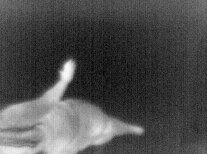
\includegraphics[scale = 0.75]{VierdeExperiment_frame}
	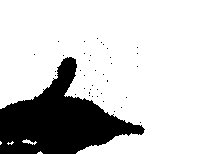
\includegraphics[scale = 0.75]{VierdeExperiment_movMask}
	\caption{frame (links) en bijhorend 'foutief' bewegingsmasker (rechts) tijdens vierde experiment}
	\label{imgRVB}
\end{figure}
De oorzaak van het probleem kan zitten in de normalisatie. Hierdoor kunnen we deze aanpassing in de code niet gebruiken. In een volgend experiment zullen we onderzoeken of het mogelijk is om de normalisatie achterwege te laten.
 
 \section{Pixelwaarde zonder normalisatie}
 \label{ERefPZN}
Dit experiment wordt in drie delen besproken. Als eerst verklaren we het doel van het experiment \ref{ERefPZND}, gevolgd door de uitwerking van het experiment en de bekomen resultaten \ref{ERefPZNV}. We sluiten af met het bespreken van de resultaten en het nemen van besluiten \ref{ERefPZNB} op het einde van het einde van het experiment.

\subsection{Doel van het experiment}
\label{ERefPZND}
Het doel van het experiment is na gaan of het mogelijk is de normalisatie stap achterwege te laten. Voor we dit onderzoeken, moeten we natuurlijk ook weten wat juist het doel is van de normalisatie stap. Tijdens de normalisatie worden de pixelwaarden verschaalt, de laagste waarde, krijgt de laagste meegegeven waarde met de functie, in ons geval is dit 0. De grootste waarde van het frame krijgt de andere meegegeven waarde, bij ons 65535. De tussenliggende waarden worden vervolgens hiertussen geschaald. Hierdoor krijgen we soms de indruk dat pixels warmer zijn geworden terwijl dit niet is. Dit geeft eveneens problemen met een leeg bed, omdat de temperatuur dan overal ongeveer gelijk is, worden kleine verschillen ineens heel groot weergegeven worden.
 
 \subsection{Uitwerking van het experiment}
 \label{ERefPZNV}
We hebben dit experiment in drie delen gedaan, dit met een paar kleine verschillen in de uitvoering.
De werking van het eerste experiment is heel eenvoudig. We halen een frame binnen, we doen deze keer de normalisatie stap niet. We lopen \'e\'en voor \'e\'en door alle pixels. We zoeken de minimale, maximale pixelwaarde en drukken deze af. We berekenen eveneens de gemiddelde pixelwaarde en drukken deze eveneens op het scherm af. \\
We doen dit eerst een paar keer voor een leeg bed, zodat we de waarden voor de achtergrond weten. Vervolgens doen we dit een paar keer voor een frame terwijl er een persoon in het bed ligt. De persoon gebruikt geen deken, bijgevolg zou voor de camera het volledige lichaam zichtbaar moeten zijn.  Vervolgens gaan we de waarden bekijken en hieruit besluiten trekken. \\
Daarna hebben we hetzelfde experiment nog eens uitgevoerd. Omdat we een paar gegevens ontbreken om correcte besluiten te kunnen trekken. We gaan nu ook berekenen hoeveel keer de maximale en minimale waarde voorkomt. Deze twee waarden worden eveneens op het scherm weergegeven. Een ander verschil is dat we tijdens de tweede poging ook de waarden bepalen van een frame waar een persoon onder een laken ligt. Dit omdat in 's nachts de pati\"enten ook onder een laken ligt en ons programma in dergelijke omgeving ook moet kunnen werken. \\
Tijdens het derde experiment, gaan we de waarden niet meer weergeven op het scherm, maar gaan we proberen om een masker te cre\"eren. Dit willen we doen door gebruik te maken van de functie createMask van de klasse DetectNotNormalized. Ook hier doen we dit voor drie verschillende toestanden, namelijk een leeg bed, een bed met een persoon en een bed met persoon met laken. Aan de hand van de verkregen maskers kunnen we dan besluiten of we met deze methode verder willen werken.
 
 
 \subsection{Bespreking resultaten en besluiten na het experiment}
 \label{ERefPZNB}
 We hebben voor de duidelijkheid dit deel van de bespreking opgesplitst in die delen. Dit zodat u het verschil in resultaten van de verschillende experimenten duidelijk kan zien. 
 
\subsubsection{Eerste poging} 
\begin{table}[hbp]
	\caption{Gemeten niet genormaliseerde waarden leeg bed, eerste poging}		
	\begin{tabular}{|c|c|c|}	
		\hline
		maximale pixelwaarde & minimale pixelwaarde & gemiddelde pixelwaarde \\ \hline
		204 & 30 & 79 \\ \hline
		189 & 17 & 75 \\ \hline
		197 & 10 & 71 \\ \hline
		255 & 0 & 73 \\ \hline
		255 & 0 & 74 \\ \hline
		254 & 6 & 69 \\ \hline
		204 & 37 & 82 \\ \hline
		255 & 0 & 64 \\ \hline
		190 & 5 & 71 \\ \hline
		255 & 0 & 59 \\ \hline
		198 & 48 & 84 \\ \hline
		206 & 40 & 82 \\ \hline
		173 & 3 & 64 \\ \hline
		190 & 1 & 66 \\ \hline
	\end{tabular}
	\label{refTabPZNL}
\end{table}
Een overzicht van de maximale, minimale en gemiddelde waarde voor een leeg bed, vindt u terug in tabel \ref{refTabPZNL}. Vervolgens hebben we de gemiddelde waarde berekend van de gemiddelde waarden, voor het leeg bed bedraagt deze 72,42. We hebben deze berekend omdat dit voor beiden gemakkelijk te berekenen en te vergelijken is. 

Vervolgens vindt u een overzicht van de maximale, minimale en gemiddelde waarde voor een bed met daarin een persoon zonder deken terug in tabel \ref{refTabPZNP}. Hier bedraagt de gemiddelde waarde van de gemiddelde waarden 83,79. \\
Als we de waarden bekijken, zien we dat als er een persoon aanwezig is, de maximale en minimale waarde altijd 255 en 0 is. Al zou normaal de aanwezigheid van een persoon de minimale waarde niet mogen be\"invloeden. Verder zien we dat de gemiddelde waarde ook hoger ligt. Maar omdat er bij het lege bed een aantal uitschieters naar boven zijn, en bij het bed met persoon een aantal uitschieters naar beneden, kunnen we hier niet alleen naar kijken. Daarom zijn zij in het tweede deel van dit experiment gaan tellen hoeveel keer de verschillende waarde voorkomt.

\begin{table}[hbp]
	\caption{Gemeten niet genormaliseerde waarden bed met persoon, eerste poging}
	\begin{tabular}{|c|c|c|}
		\hline
		maximale pixelwaarde & minimale pixelwaarde & gemiddelde pixelwaarde \\ \hline
		255 & 0 & 82 \\ \hline
		255 & 0 & 78 \\ \hline
		255 & 0 & 80 \\ \hline
		255 & 0 & 84 \\ \hline
		255 & 0 & 91 \\ \hline
		255 & 0 & 88 \\ \hline
		255 & 0 & 89 \\ \hline
		255 & 0 & 92 \\ \hline
		255 & 0 & 89 \\ \hline
		255 & 0 & 89 \\ \hline
		255 & 0 & 77 \\ \hline
		255 & 0 & 83 \\ \hline
		255 & 0 & 75 \\ \hline
		255 & 0 & 76 \\ \hline
	\end{tabular}
	
	\label{refTabPZNP}
\end{table}

\subsubsection{Tweede poging}
\begin{table}[hbp]
	\caption{Gemeten niet genormaliseerde waarden leeg bed, tweede experiment}
	\begin{tabular}{|c|c|c|c|c|}
		\hline
		maximale waarde & minimale waarde & gemiddelde waarde & aantal maximaal & aantal minimaal\\ \hline
		202 & 21 & 78 & 1 & 1\\ \hline
		188 & 18 & 74 & 1 & 1\\ \hline
		196 & 39 & 83 & 1 & 1 \\ \hline
		208 & 39 & 83 & 1 & 1 \\ \hline
		193 & 25 & 77 & 1 & 1 \\ \hline
		207 & 36 & 84 & 1 & 1 \\ \hline
		255 & 0  & 61 & 6 & 8 \\ \hline
		211 & 39 & 82 & 1 & 3 \\ \hline
		182 & 9  & 73 & 1 & 1 \\ \hline
		202 & 28 & 78 & 1 & 1 \\ \hline
		185 & 10 & 72 & 1 & 1 \\ \hline
		197 & 15 & 75 & 1 & 1 \\ \hline
		174 & 3  & 67 & 1 & 1 \\ \hline
		200 & 30 & 81 & 1 & 1 \\ \hline
		255 & 0  & 60 & 2 & 11\\ \hline
	\end{tabular}
	\label{refTabPZNLT}
\end{table}

De gemeten pixelwaarden voor het lege bed ziet u in tabel \ref{refTabPZNLT}. Ook hier hebben we de gemiddelde gemiddelde pixelwaarde berekend. Deze bedraagt nu 75,2. Hoe kan het dat deze ineens warmer is? Volgens ons komt dit door een aantal factoren. Het tweede experiment gebeurde later op de dag, daardoor was de kamer door de zon meer opgewarmd, verder stonden in dezelfde kamer ook twee computers aan. Deze zorgden ook voor meer omgevingswarmte. We zien wel weinig verschil in de extremen. \\
\begin{table}[hbp]
	\caption{Gemeten niet genormaliseerde waarden bij een bed met persoon zonder laken, tweede experiment}
	\begin{tabular}{|c|c|c|c|c|}
		\hline
		maximale waarde & minimale waarde & gemiddelde waarde & aantal maximaal & aantal minimaal \\ \hline
		255 & 0 & 100 & 12 & 19 \\ \hline
		255 & 0 & 106 & 11 & 9  \\ \hline
		255 & 0 & 105 & 26 & 29 \\ \hline
		255 & 0 & 96  & 7  & 6 \\ \hline
		255 & 0 & 107 & 73 & 51  \\ \hline
		255 & 0 & 104 & 40 & 46 \\ \hline
		255 & 0 & 103 & 42 & 46 \\ \hline
		255 & 0 & 102 & 45 & 44 \\ \hline
		255 & 0 & 89  & 22 & 21 \\ \hline
		255 & 0 & 104 & 11 & 20 \\ \hline
		255 & 0 & 96  & 9  & 7 \\ \hline
		255 & 0 & 96  & 8  & 15 \\ \hline
		255 & 0 & 86  & 7  & 13  \\ \hline
		255 & 0 & 94  & 11 & 13 \\ \hline
		255 & 0 & 94  & 4  & 6  \\ \hline
	\end{tabular}
	\label{refTabPZNPT}
\end{table}

De waarden voor het bed met een persoon zonder laken ziet u in tabel \ref{refTabPZNPT},hier bedraagt de gemiddelde gemiddelde pixelwaarde 86,33. Deze waarde is ongeveer evenveel gestegen als de gemiddelde waarde bij een leeg bed. Dit komt natuurlijk door dezelfde factoren. Hier valt natuurlijk direct op dat de maxima en minima weer elke keer gelijk zijn. De extremen zijn precies extremer geworden. Verder zien we ook dat de maximale en minimale waarden beduidend meer voorkomen. \\
Als laatste hebben we ook de resultaten van de frames van een persoon met laken samengevoegd in tabel \ref{refTabPZNPL}. Uit deze waarden bepaalden we de gemiddelde gemiddelde pixelwaarde, deze bedraagt 98,8. Deze is beduidend hoger dan de pixelwaarde voor een persoon zonder laken. Dit komt volgens ons doordat de het laken de lichaamswarmte meer verspreid. Daardoor dat ook het aantal pixels met een maximale waarde stijgt. \\
Uit dit experiment kunnen we natuurlijk geen definitief besluit trekken, hiervoor zijn 15 steekproeven niet voldoende. Het geeft echter aan dat we in deze richting mogelijk wel verder kunnen. Maar hiervoor moeten eerst andere onderzoeken en experimenten gebeuren. Dit hebben we dan ook gedaan in het derde experiment.
\begin{table}[hbp]
	\caption{Gemeten niet genormaliseerde waarden bij een bed met persoon met laken, tweede experiment}
	\begin{tabular}{|c|c|c|c|c|}
		\hline
		maximale waarde & minimale waarde & gemiddelde waarde & aantal maximaal & aantal minimaal \\ \hline
		255 & 0 & 99 & 19 & 28 \\ \hline
		255 & 0 & 89 & 14 & 20 \\ \hline
		255 & 0 & 93 & 18 & 19 \\ \hline
		255 & 0 & 95 & 20 & 23 \\ \hline
		255 & 0 & 88 & 17 & 22 \\ \hline
		255 & 0 & 88 & 22 & 22 \\ \hline
		255 & 0 & 91 & 21 & 22 \\ \hline
		255 & 0 & 86 & 19 & 17 \\ \hline
		255 & 0 & 85 & 19 & 23 \\ \hline
		255 & 0 & 83 & 6  & 10 \\ \hline
		255 & 0 & 72 & 35 & 37 \\ \hline
		255 & 0 & 78 & 15 & 23 \\ \hline
		255 & 0 & 77 & 16 & 9  \\ \hline
		255 & 0 & 86 & 27 & 16 \\ \hline
		255 & 0 & 85 & 8  & 6  \\ \hline
	\end{tabular}
	
	\label{refTabPZNPL}
\end{table}

\subsubsection{Derde poging}  
\begin{figure}[hbp]
	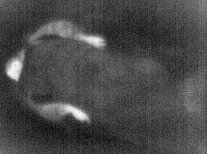
\includegraphics[scale = 0.75]{NotNormalizedFrame}
	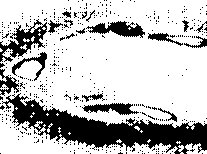
\includegraphics[scale = 0.75]{NotNormalizedMask}
	\caption{frame (links) en bijhorend masker (rechts) bepaald door niet genormaliseerde waarden}
	\label{imgNGn}
\end{figure}

Door de klasse Detect aan te passen, hebben we dit verder onderzocht.  We hebben geprobeerd om zo maskers te maken. Een voorbeeld van zo een masker ziet u terug in figuur \ref{imgNGn}.  Links ziet u het frame, om dit op te slagen zijn de waarde wel genormaliseerd, anders krijg je een volledig grijs frame te zien. Links ziet u het berekende masker bij het frame.  Zoals u kan zien, geeft dit niet de gewenste resultaten. Omdat er een veel groter deel dan enkel de persoon wit wordt. Dit werd niet beter door het aanpassen van de threshold. Daarom hebben we moeten besluiten dat het niet mogelijk is om dit te gebruiken. Het voordeel hiervan is wel dat je rechtstreeks met life beelden kunt werken. Maar doordat de camera \ref{MRefIRC} een warmtebereik heeft van -40 tot 330 graden, is het verschil tussen kamertemperatuur en de lichaamstemperatuur niet groot genoeg. Hierdoor gebeurden valse detecties. De normalisatie stap is dus nodig om dit verschil in temperatuur te vergroten.
 
 \section{Hoofd gebaseerde detectie}
 \label{ERefHGD}
 Dit idee komt voor uit de gedachte dat het hoofd altijd zichtbaar is. Verder zagen we uit de voorgaande resultaten dat we het interessant kan zijn om een keer opnieuw te beginnen en deze keer vanuit een ander oogpunt te werken. Dit experiment wordt ook in verschillende delen besproken. We beginnen met het uitleggen van het doel van het experiment \ref{ERefHGDD}, dit wordt gevolg door de verduidelijking van de uitwerking van het experiment \ref{ERefHGDU}. Als laatste bespreken we de resultaten en de daaruit genomen besluiten \ref{ERefHGDB}.
 
 \subsection{Doel van het experiment}
 \label{ERefHGDD}
 Het doel van dit experiment is nagaan of het mogelijk is door om aan de hand van de locatie van het hoofd te bepalen of een persoon al dan niet uit bed probeert te stappen.
 
 \subsection{Uitwerking van het experiment}
 \label{ERefHGDU}
 Dit experiment bestaat uit twee delen, eerst hebben we een sequentie van beelden openomen waarop een persoon te zien is die een paar keer in en uit een bed stapt. Dit een paar keer zonder een deken en een paar keer met een deken. Nadat deze beelden gemaakt en opgeslagen zijn, gaan we ze een terug ophalen en met behulp van de mouseCallBack functie die eerst verklaard werd, gaan we ongeveer op het midden van het zichtbare deel van het hoofd klikken. Deze waarden worden genoteerd en samengevoegd in een grafiek, later worden hier besluiten uit genomen. 
 
 \subsection{Resultaten en besluiten van het experiment}
 \label{ERefHGDB}
Zoals eerder vermeld hebben we de waarden van de co\"orniaten in een grafiek gegoten, de grafiek voor de eerste keer in en uit een bed stappen, ziet u in figuur \ref{imgCHZ}.
\begin{figure}[hbp]
	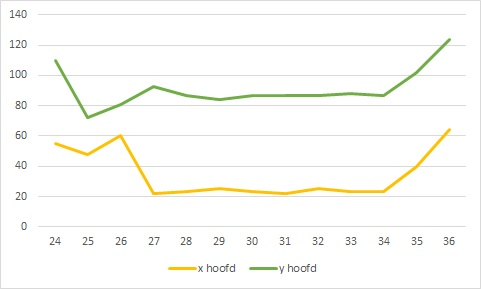
\includegraphics[scale = 0.75]{Grafiek_UitBedZ}
	\caption{Grafiek met de co\"ordinaten van het hoofd (eerste set frames), met op de horizontale as de framenummers, de verticale de waarden}
	\label{imgCHZ}
\end{figure}
Hier valt direct op dat tussen frame 24 en 27 de persoon bezig is met te gaan liggen, hier zijn de waarden voor de co\"ordinaten groot, tussen frame 28 en 34 ligt de persoon in bed en blijven de waarden ongeveer gelijk, later tussen frame 34 en 36 staat de persoon op en worden de waarden weer groter. We zullen moeten zien of deze resultaten ook bij de andere drie metingen terug komen. We zien ook dat de waarden voor de y-co\"ordinaat ongeveer gelijk blijven, deze zullen we niet kunnen gebruiken voor de detectie. \\
De grafiek van de tweede reeks frames ziet u in figuur \ref{imgCHZT}.
\begin{figure}[hbp]
	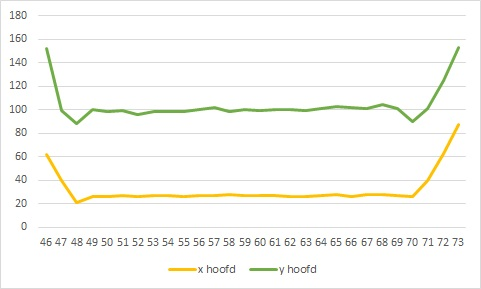
\includegraphics[scale = 0.75]{Grafiek_UitBedZT}
	\caption{Grafiek met de co\"ordinaten van het hoofd (tweede set frames), met op de horizontale as de framenummers, de verticale de waarden}
	\label{imgCHZT}
\end{figure}
Uit deze waarden kunnen we dezelfde besluiten trekken. \\
De derde en vierde set zijn frames van een persoon met laken, al heeft dat voor deze test geen invloed. De resultaten van de derde set ziet u terug in figuur \ref{imgCHM}. \\
\begin{figure}[hbp]
	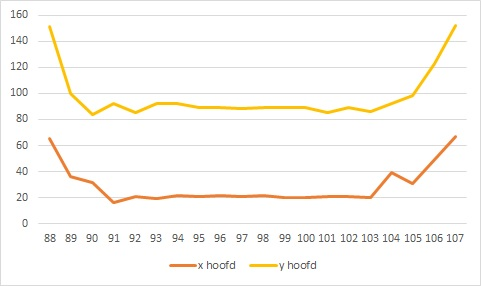
\includegraphics[scale = 0.75]{Grafiek_UitBedM}
	\caption{Grafiek met de co\"ordinaten van het hoofd (derde set frames), met op de horizontale as de framenummers, de verticale de waarden}
	\label{imgCHM}
\end{figure}
De grafiek van de vierde sequentie van frames ziet u terug in figuur \ref{imgCHMT}.
\begin{figure}[hbp]
	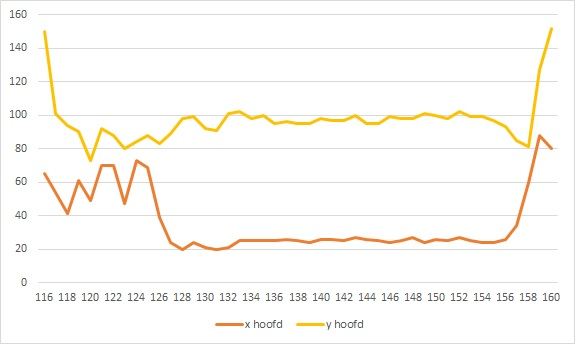
\includegraphics[scale = 0.75]{Grafiek_UitBedMT}
	\caption{Grafiek met de co\"ordinaten van het hoofd (vierde set frames), met op de horizontale as de framenummers, de verticale de waarden}
	\label{imgCHMT}
\end{figure}
Hier ziet u in het begin een paar schommelingen in de waarden. Dit komt doordat de persoon een paar keer terug recht is gekomen om het deken goed te leggen. Verder zien we dat de besluiten die we namen na de eerste set hier ook nog geldig zijn.\\
In het algemeen kunnen we dit experiment afsluiten met het besluit dat het zinvol is dit verder te bekijken. Zoals bijvoorbeeld te bepalen hoe de co\"ordinaten zich verhouden met de hoeken van het bed. Verder moeten we ook nog bekijken of het mogelijk is om met een soort van blobdetectie het midden van het hoofd te berekenen en of we dan geen valse detecties krijgen door de restwarmte.

\chapter{Algemeen besluit}
Het systeem detecteerd goed langs welke zijde er uit het bed gestapt wordt. Een mogelijk uitbereiding is de timer van hoelang een persoon uit bed is. Momenteel lukt dit nog niet door de restwarmte van het bed. Indien er ook wenst gewerkt te worden zonder de afbeeldingen op te slagen moet er ook nog aan de code gewerkt worden. De beelden die door de camera worden geleverd staan in een ander formaat als de beelden die ik verwerk, bijgevolg moeten er dan nog een paar kleine aanpassingen gebeuren. Verder kan er ook nog onderzoek gebruiken naar het gebruik van een night vision camera, om het probleem van de restwarmte te verkleinen. Verder kunnen ook andere cameras eens getest worden, de meeste mensen klagen over het klikgeluidje dat de camera maakt.